%Version 3.1 December 2024
% See section 11 of the User Manual for version history
%
%%%%%%%%%%%%%%%%%%%%%%%%%%%%%%%%%%%%%%%%%%%%%%%%%%%%%%%%%%%%%%%%%%%%%%
%%                                                                 %%
%% Please do not use \input{...} to include other tex files.       %%
%% Submit your LaTeX manuscript as one .tex document.              %%
%%                                                                 %%
%% All additional figures and files should be attached             %%
%% separately and not embedded in the \TeX\ document itself.       %%
%%                                                                 %%
%%%%%%%%%%%%%%%%%%%%%%%%%%%%%%%%%%%%%%%%%%%%%%%%%%%%%%%%%%%%%%%%%%%%%

%%\documentclass[referee,sn-basic]{sn-jnl}% referee option is meant for double line spacing

%%=======================================================%%
%% to print line numbers in the margin use lineno option %%
%%=======================================================%%

%%\documentclass[lineno,pdflatex,sn-basic]{sn-jnl}% Basic Springer Nature Reference Style/Chemistry Reference Style

%%=========================================================================================%%
%% the documentclass is set to pdflatex as default. You can delete it if not appropriate.  %%
%%=========================================================================================%%

%%\documentclass[sn-basic]{sn-jnl}% Basic Springer Nature Reference Style/Chemistry Reference Style

%%Note: the following reference styles support Namedate and Numbered referencing. By default the style follows the most common style. To switch between the options you can add or remove “Numbered” in the optional parenthesis. 
%%The option is available for: sn-basic.bst, sn-chicago.bst%  
 
%%\documentclass[pdflatex,sn-nature]{sn-jnl}% Style for submissions to Nature Portfolio journals
%%\documentclass[pdflatex,sn-basic]{sn-jnl}% Basic Springer Nature Reference Style/Chemistry Reference Style
\documentclass[pdflatex,sn-mathphys-num]{sn-jnl}% Math and Physical Sciences Numbered Reference Style
%%\documentclass[pdflatex,sn-mathphys-ay]{sn-jnl}% Math and Physical Sciences Author Year Reference Style
%%\documentclass[pdflatex,sn-aps]{sn-jnl}% American Physical Society (APS) Reference Style
%%\documentclass[pdflatex,sn-vancouver-num]{sn-jnl}% Vancouver Numbered Reference Style
%%\documentclass[pdflatex,sn-vancouver-ay]{sn-jnl}% Vancouver Author Year Reference Style
%%\documentclass[pdflatex,sn-apa]{sn-jnl}% APA Reference Style
%%\documentclass[pdflatex,sn-chicago]{sn-jnl}% Chicago-based Humanities Reference Style

%%%% Standard Packages
%%<additional latex packages if required can be included here>

\usepackage{graphicx}%
\usepackage{multirow}%
\usepackage{amsmath,amssymb,amsfonts}%
\usepackage{amsthm}%
\usepackage{mathrsfs}%
\usepackage[title]{appendix}%
\usepackage{xcolor}%
\usepackage{textcomp}%
\usepackage{manyfoot}%
\usepackage{booktabs}%
\usepackage{algorithm}%
\usepackage{algorithmicx}%
\usepackage{algpseudocode}%
\usepackage{listings}%

\usepackage{kotex}
%%%%

%%%%%=============================================================================%%%%
%%%%  Remarks: This template is provided to aid authors with the preparation
%%%%  of original research articles intended for submission to journals published 
%%%%  by Springer Nature. The guidance has been prepared in partnership with 
%%%%  production teams to conform to Springer Nature technical requirements. 
%%%%  Editorial and presentation requirements differ among journal portfolios and 
%%%%  research disciplines. You may find sections in this template are irrelevant 
%%%%  to your work and are empowered to omit any such section if allowed by the 
%%%%  journal you intend to submit to. The submission guidelines and policies 
%%%%  of the journal take precedence. A detailed User Manual is available in the 
%%%%  template package for technical guidance.
%%%%%=============================================================================%%%%

%% as per the requirement new theorem styles can be included as shown below
\theoremstyle{thmstyleone}%
\newtheorem{theorem}{Theorem}%  meant for continuous numbers
%%\newtheorem{theorem}{Theorem}[section]% meant for sectionwise numbers
%% optional argument [theorem] produces theorem numbering sequence instead of independent numbers for Proposition
\newtheorem{proposition}[theorem]{Proposition}% 
%%\newtheorem{proposition}{Proposition}% to get separate numbers for theorem and proposition etc.

\theoremstyle{thmstyletwo}%
\newtheorem{example}{Example}%
\newtheorem{remark}{Remark}%

\theoremstyle{thmstylethree}%
\newtheorem{definition}{Definition}%

\raggedbottom
%%\unnumbered% uncomment this for unnumbered level heads

\begin{document}

\title[Article Title]{Live Mobile Learning System with Multi-Room and Whiteboard Features}

%%=============================================================%%
%% GivenName	-> \fnm{Joergen W.}
%% Particle	-> \spfx{van der} -> surname prefix
%% FamilyName	-> \sur{Ploeg}
%% Suffix	-> \sfx{IV}
%% \author*[1,2]{\fnm{Joergen W.} \spfx{van der} \sur{Ploeg} 
%%  \sfx{IV}}\email{iauthor@gmail.com}
%%=============================================================%%

\author*{\fnm{Hosung} \sur{Kim}}\email{hosungkim5108@gmail.com}

%%\author[2,3]{\fnm{Second} \sur{Author}}\email{iiauthor@gmail.com}
%%\equalcont{These authors contributed equally to this work.}

%%\author[1,2]{\fnm{Third} \sur{Author}}\email{iiiauthor@gmail.com}
%%\equalcont{These authors contributed equally to this work.}

\affil{\orgdiv{Department of Computer Engineering}, \orgname{Hongik University}, \orgaddress{ \city{Seoul}, \country{Korea}}}

\abstract{본 보고서는 기존의 단일 강의실 기반 동기식 모바일 원격 교육 시스템을 확장하여, 보다 실질적인 교육 환경을 지원하는 프로토타입 시스템을 설계하고 구현한 내용을 다룬다. 기존 시스템이 제공하던 채팅, 음성 및 영상 공유, PDF 주석 기능 외에도, 본 시스템은 다중 강의실 구조, 실시간 참여자 명단, 강의자 전면 카메라 프리뷰, 화이트보드 기능을 추가하였다. 서버 측에서는 NGINX 기반 RTMP 스트리밍 서버와 WebSocket 서버를 Swift 기반으로 통합하여 실행 및 관리의 일원화를 달성하였으며, 강의실 생성, 입장, 퇴장, 채팅, 참여자 동기화 등의 기능도 추가 구현하였다. 클라이언트 측면에서는 ReplayKit을 활용하여 강의자료 영역만 선택적으로 송출하도록 개선하였다. 한편, 화이트보드와 강의자료를 동시에 표시할 수 없는 점은 사용자 경험 측면에서 한계로 작용하며, 이를 개선하기 위한 UI 설계가 향후 과제로 제시된다.}

%%\keywords{keyword1, Keyword2, Keyword3, Keyword4}

%%\pacs[JEL Classification]{D8, H51}

%%\pacs[MSC Classification]{35A01, 65L10, 65L12, 65L20, 65L70}

\maketitle

\section{Introduction}\label{sec1}

선행 보고서에서는 동기식 모바일 원격 교육 시스템에 대한 이해를 목적으로 텍스트 기반 채팅, 강사의 음성 및 영상 공유, PDF 기반 강의 자료 주석 기능 등을 포함한 데모 애플리케이션을 설계 및 구현하였다. 해당 시스템은 RTMP(Real-Time Messaging Protocol)\cite{RTMP} 및 WebSocket 기반의 통신 구조 위에 구축되었으며, 제한된 환경에서의 실시간 강의 및 상호작용 가능성을 검증하였다.

그러나 기존의 시스템은 단일 강의실과 제한된 기능으로 구성되어, 실질적인 교육 서비스로의 확장을 위해서는 기능적 보완이 요구된다. 이에 본 보고서에서는 다음과 같은 네 가지 기능을 추가로 설계 및 구현하였다. 첫째, 사용자가 직접 강의실을 생성하고 선택적으로 입장할 수 있는 다중 강의실 구조를 도입하였다. 둘째, 강의자가 실시간으로 참여자 명단을 확인할 수 있는 기능을 추가하였다. 셋째, 강의자가 송출중인 자신의 전면 카메라 화면을 실시간으로 확인할 수 있는 기능을 추가하였다. 넷째, 화이트보드 기능을 추가하였다.

\section{Design}\label{sec2}

\subsection{Structure}\label{subsec1}

\begin{figure}[h]
\centering
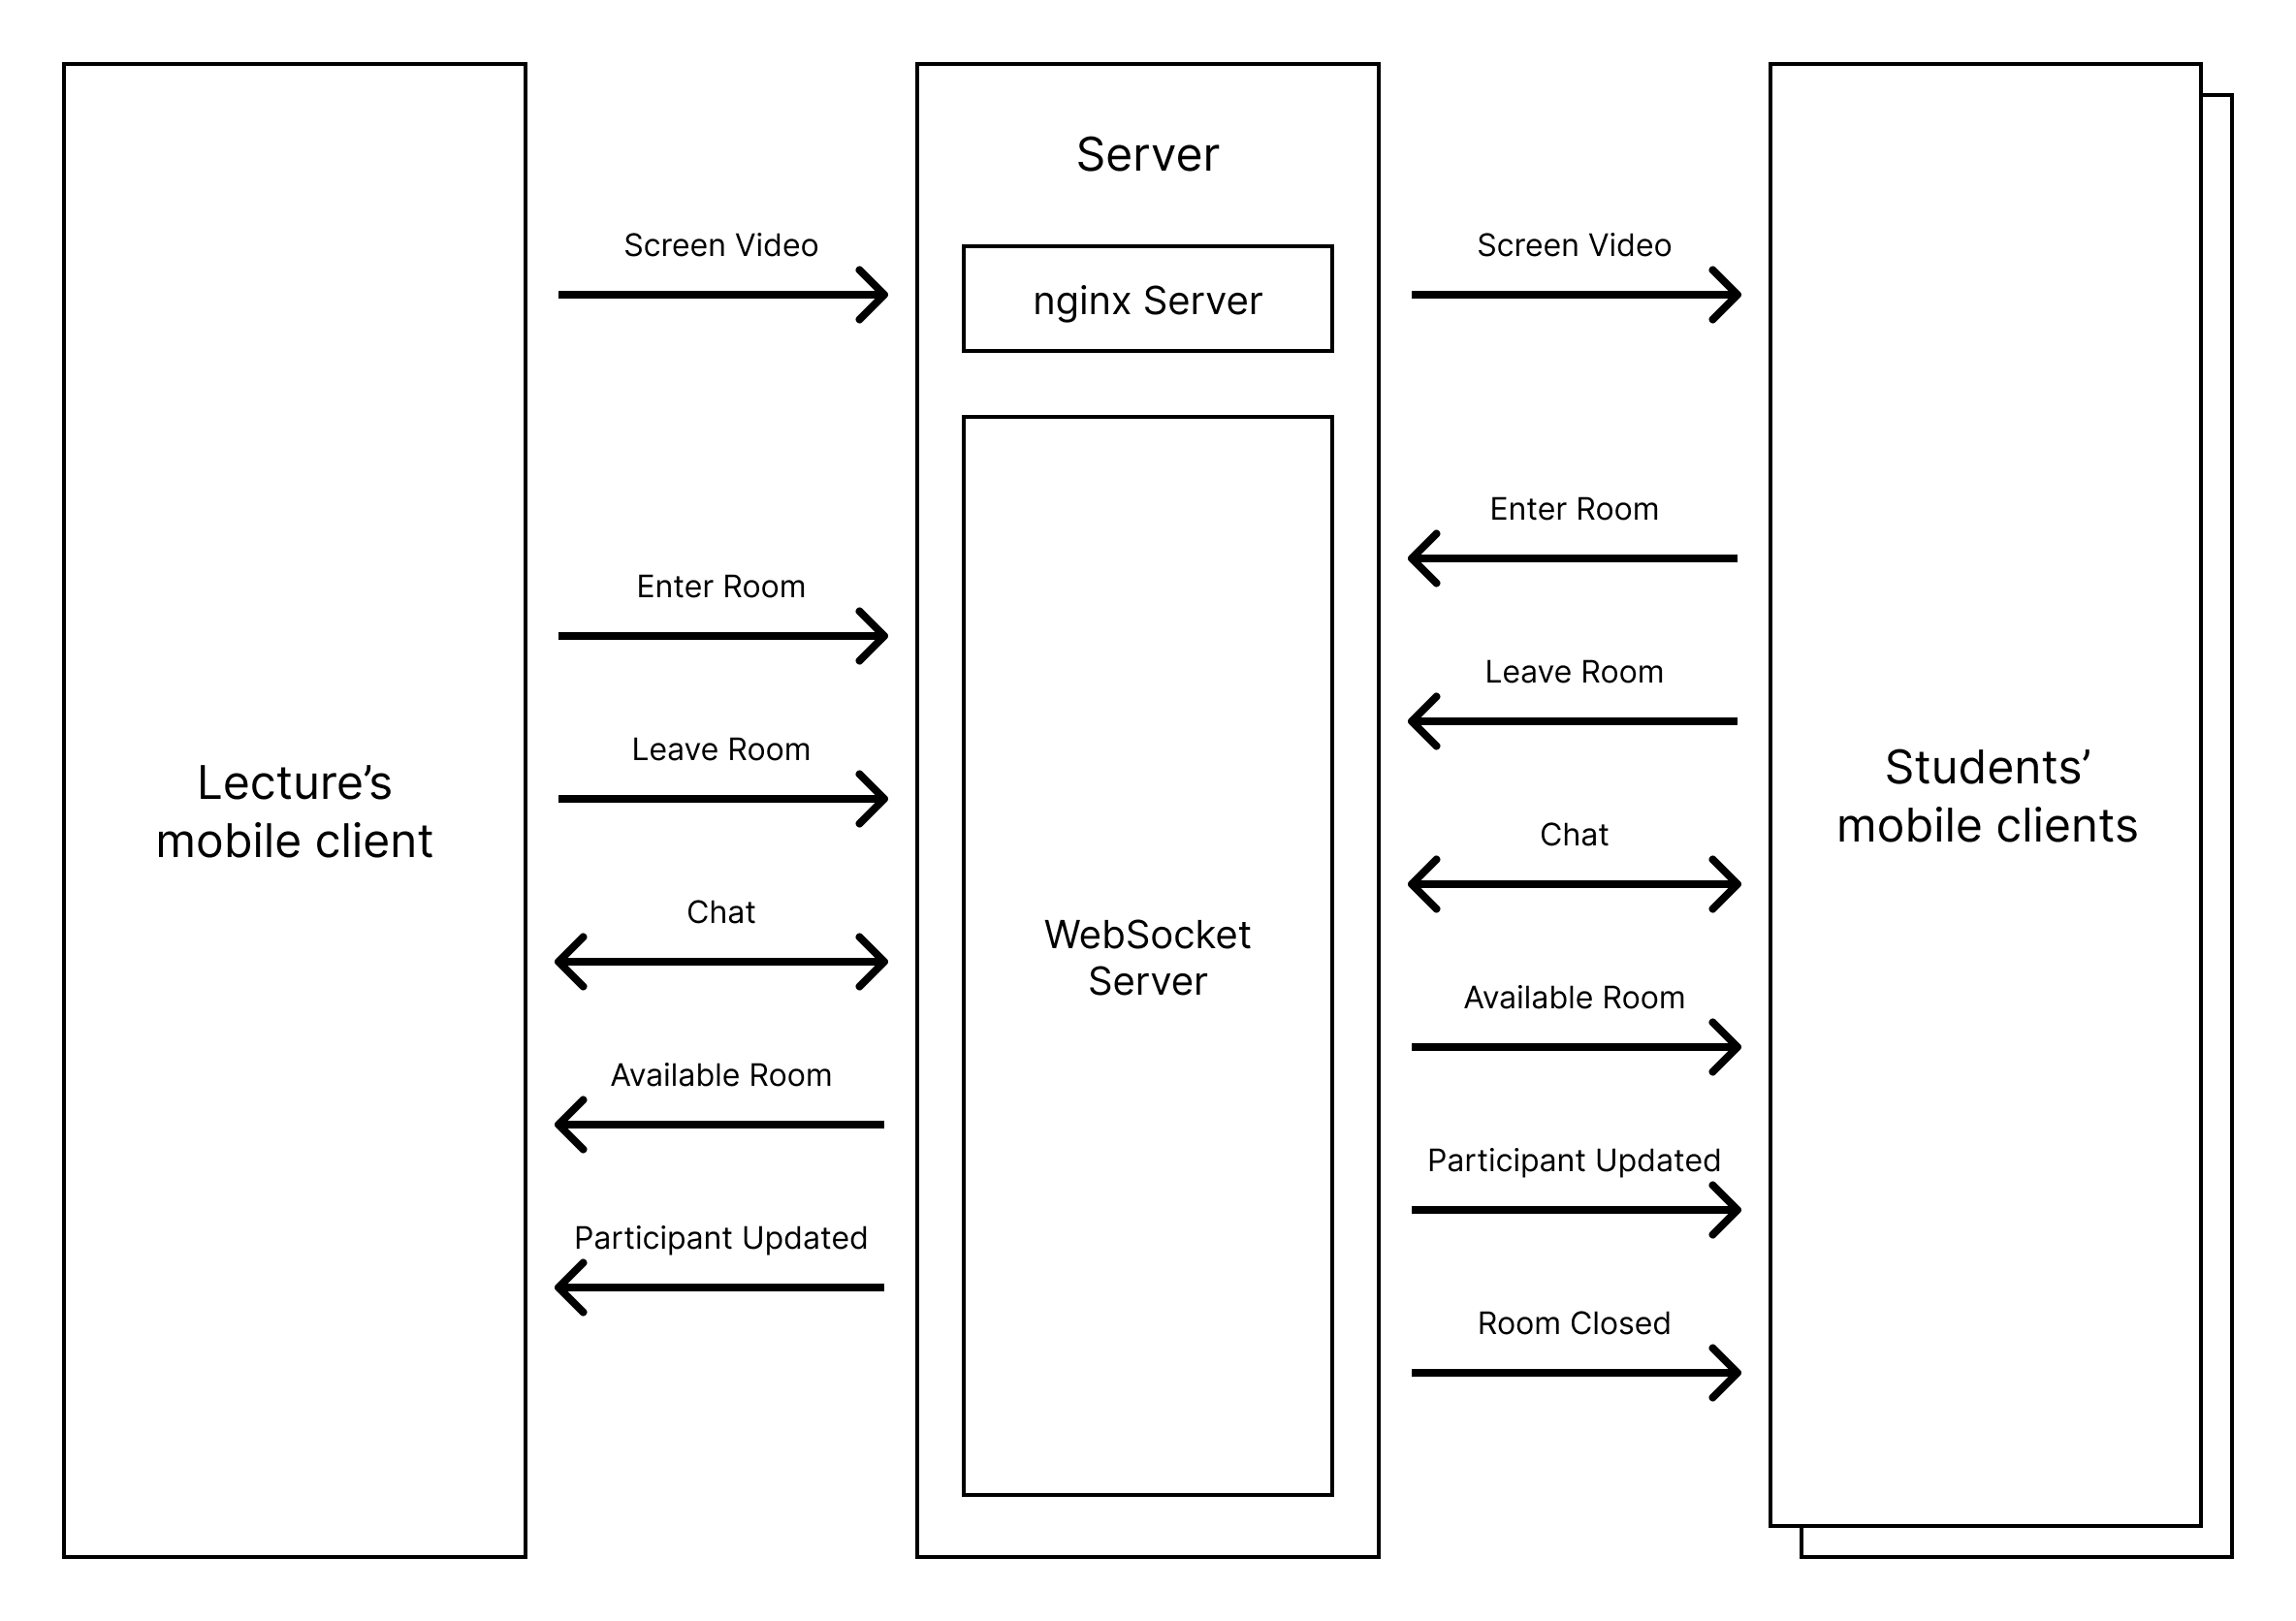
\includegraphics[width=0.9\textwidth]{architecture_of_system.png}
\caption{Structure of a system}\label{fig1}
\end{figure}

기존의 시스템은 Java Spring\cite{Spring}의 채팅 서버, NGINX\cite{NGINX}의 스트리밍 서버, iPadOS의 클라이언트로 구성되어 있어 서로 다른 환경에서 동작하였다. 이는 실행 및 테스트의 복잡성, 유지보수의 비효율성을 초래하였다. 이를 해결하기 위해 모든 프로그램을 Xcode\cite{Xcode} 기반 프로젝트 내에서 통합적으로 관리할 수 있도록 구조를 개선하였다.

한편, WebSocket 서버는 채팅 기능 뿐만 아니라 다중 강의실 기능을 지원하기 위해 확장되었다. 새로운 시스템에서는 강의실 생성, 입장 및 퇴장, 채팅, 강의실 목록 조회, 참여자 명단 동기화 등 다중 강의실 기능 전반을 담당하도록 설계하였다.

\section{Implementation}\label{sec3}

\subsection{Server}\label{subsec2}

서버는 클라이언트와의 개발 환경의 일관성을 확보하고 운영 및 유지보수의 효율성을 높이기 위해 스트리밍 서버의 실행 방식을 개선하고 WebSocket 서버를 Swift 기반으로 전면 재구현하였다.

스트리밍 서버는 기존과 동일하게 NGINX RTMP 서버를 사용하되, 실행 방식에 있어 통합이 이루어졌다. 기존에는 NGINX를 별도의 실행 환경에서 수동으로 실행해야했지만, 개선된 구조에서는 Swift 서버 실행 시 \verb+Process()+를 통해 nginx.exe와 nginx.conf 설정파일을 프로그램적으로 호출함으로써 서버 실행 및 종료를 자동화하였다. 이를 통해 두 개의 서버를 하나의 Xcode Target으로 관리할 수 있게 되어 실행 절차가 간소화되었다.

WebSocket 서버는 기존의 Java Spring 기반에서 Network Framework\cite{Network}의 \verb+NWProtocolWebSocket+을 활용한 Swift 서버로 재구현하였다. 새롭게 구현된 서버는 채팅 뿐만 아니라 강의실 입장 및 퇴장, 강의실 목록, 참여자 명단 등 강의실 관리 전반을 포괄적으로 처리할 수 있도록 하였다. 서버-클라이언트 간 통신에는 \verb+Codable+을 상속한 \verb+enum+을 사용하여 기능 확장을 용이하게 하고 다양한 종류의 메세지를 주고받을 수 있도록 하였다.

WebSocket 서버는 각 강의실을 UUID를 key로 하는 딕셔너리 형태로 관리하며, 강의실에 변화가 있을 때마다 Available Room 메세지를 모든 클라이언트에게 브로드캐스트한다. Enter Room, Leave Room 메세지를 수신받으면 해당 클라이언트를 관련 강의실에 등록하거나 제거하며, 강의자가 퇴장할 경우 해당 강의실의 모든 학생에게 Room Closed 메세지를 전송하여 강의 종료를 알린다. 또한 참여자에 변화가 있을 때마다 Participant Updated 메세지를 해당 강의실 내 모든 클라이언트에게 전송하며, 채팅 메세지는 동일 강의실 내 모든 클라이언트에게 브로드캐스트된다.

\subsection{Client}\label{subsec3}

\begin{figure}[h]
\centering
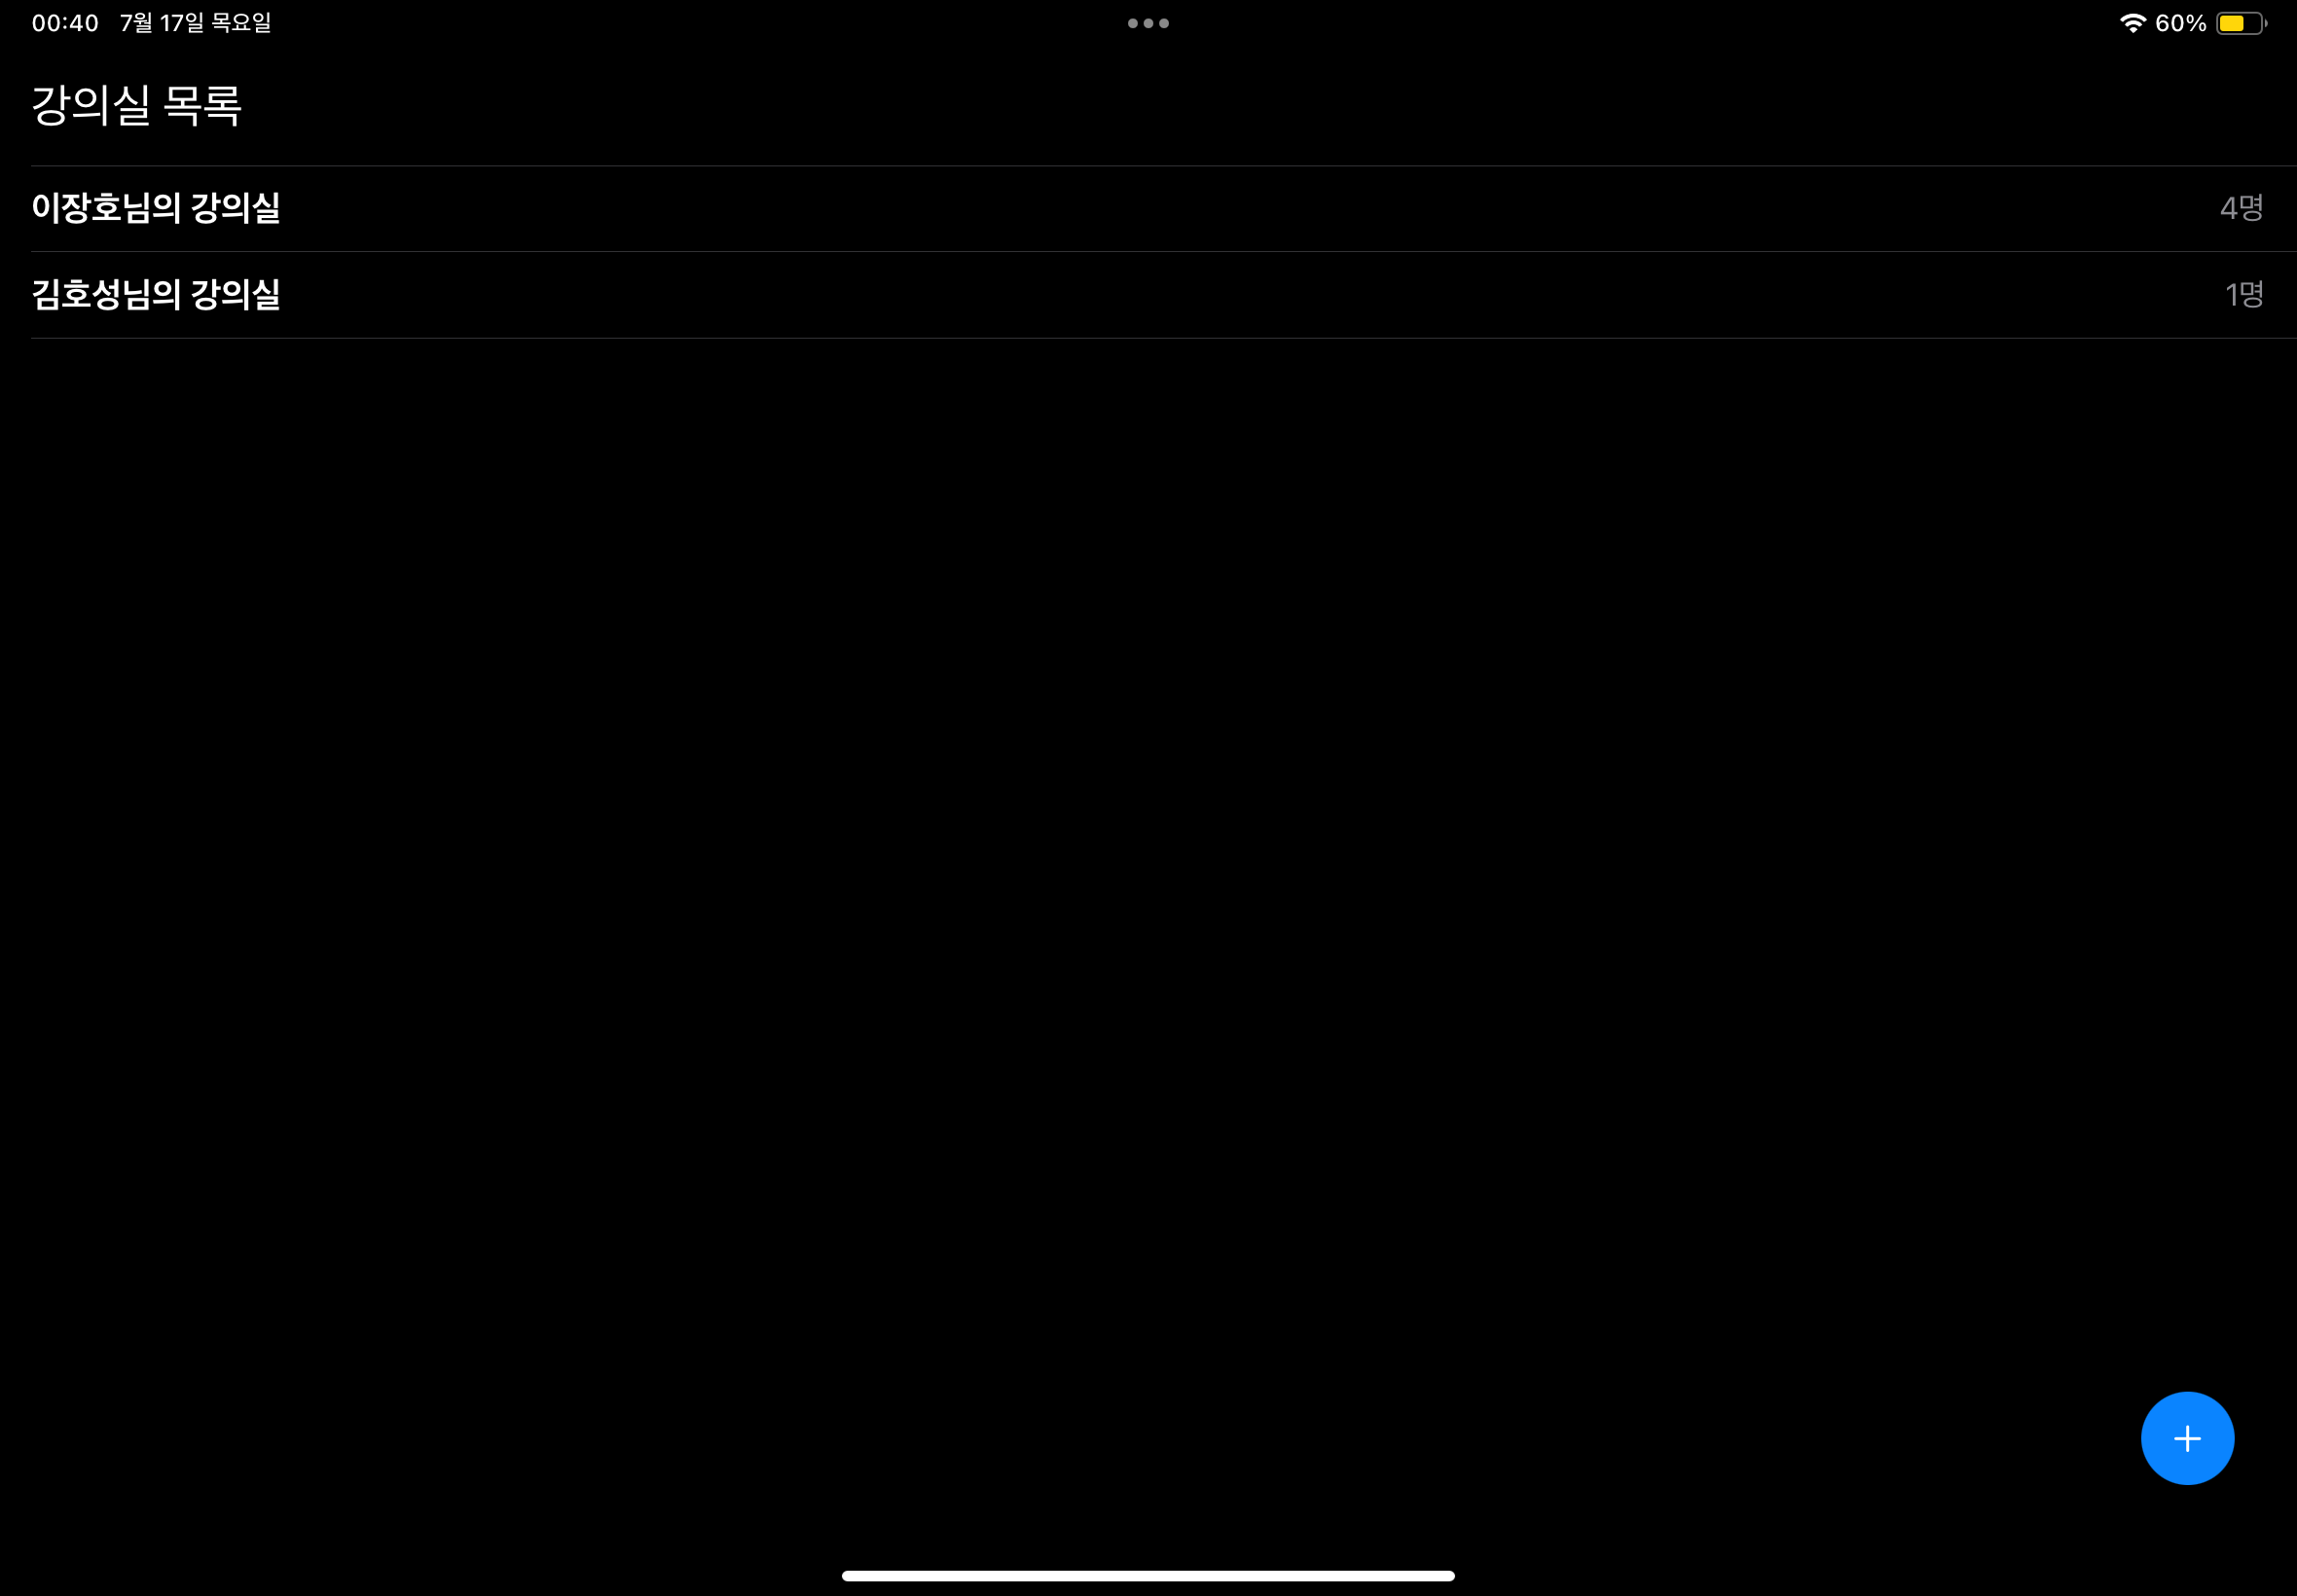
\includegraphics[width=0.9\textwidth]{home.PNG}
\caption{User interface of the home screen}\label{fig2}
\end{figure}

\begin{figure}[p]
\centering
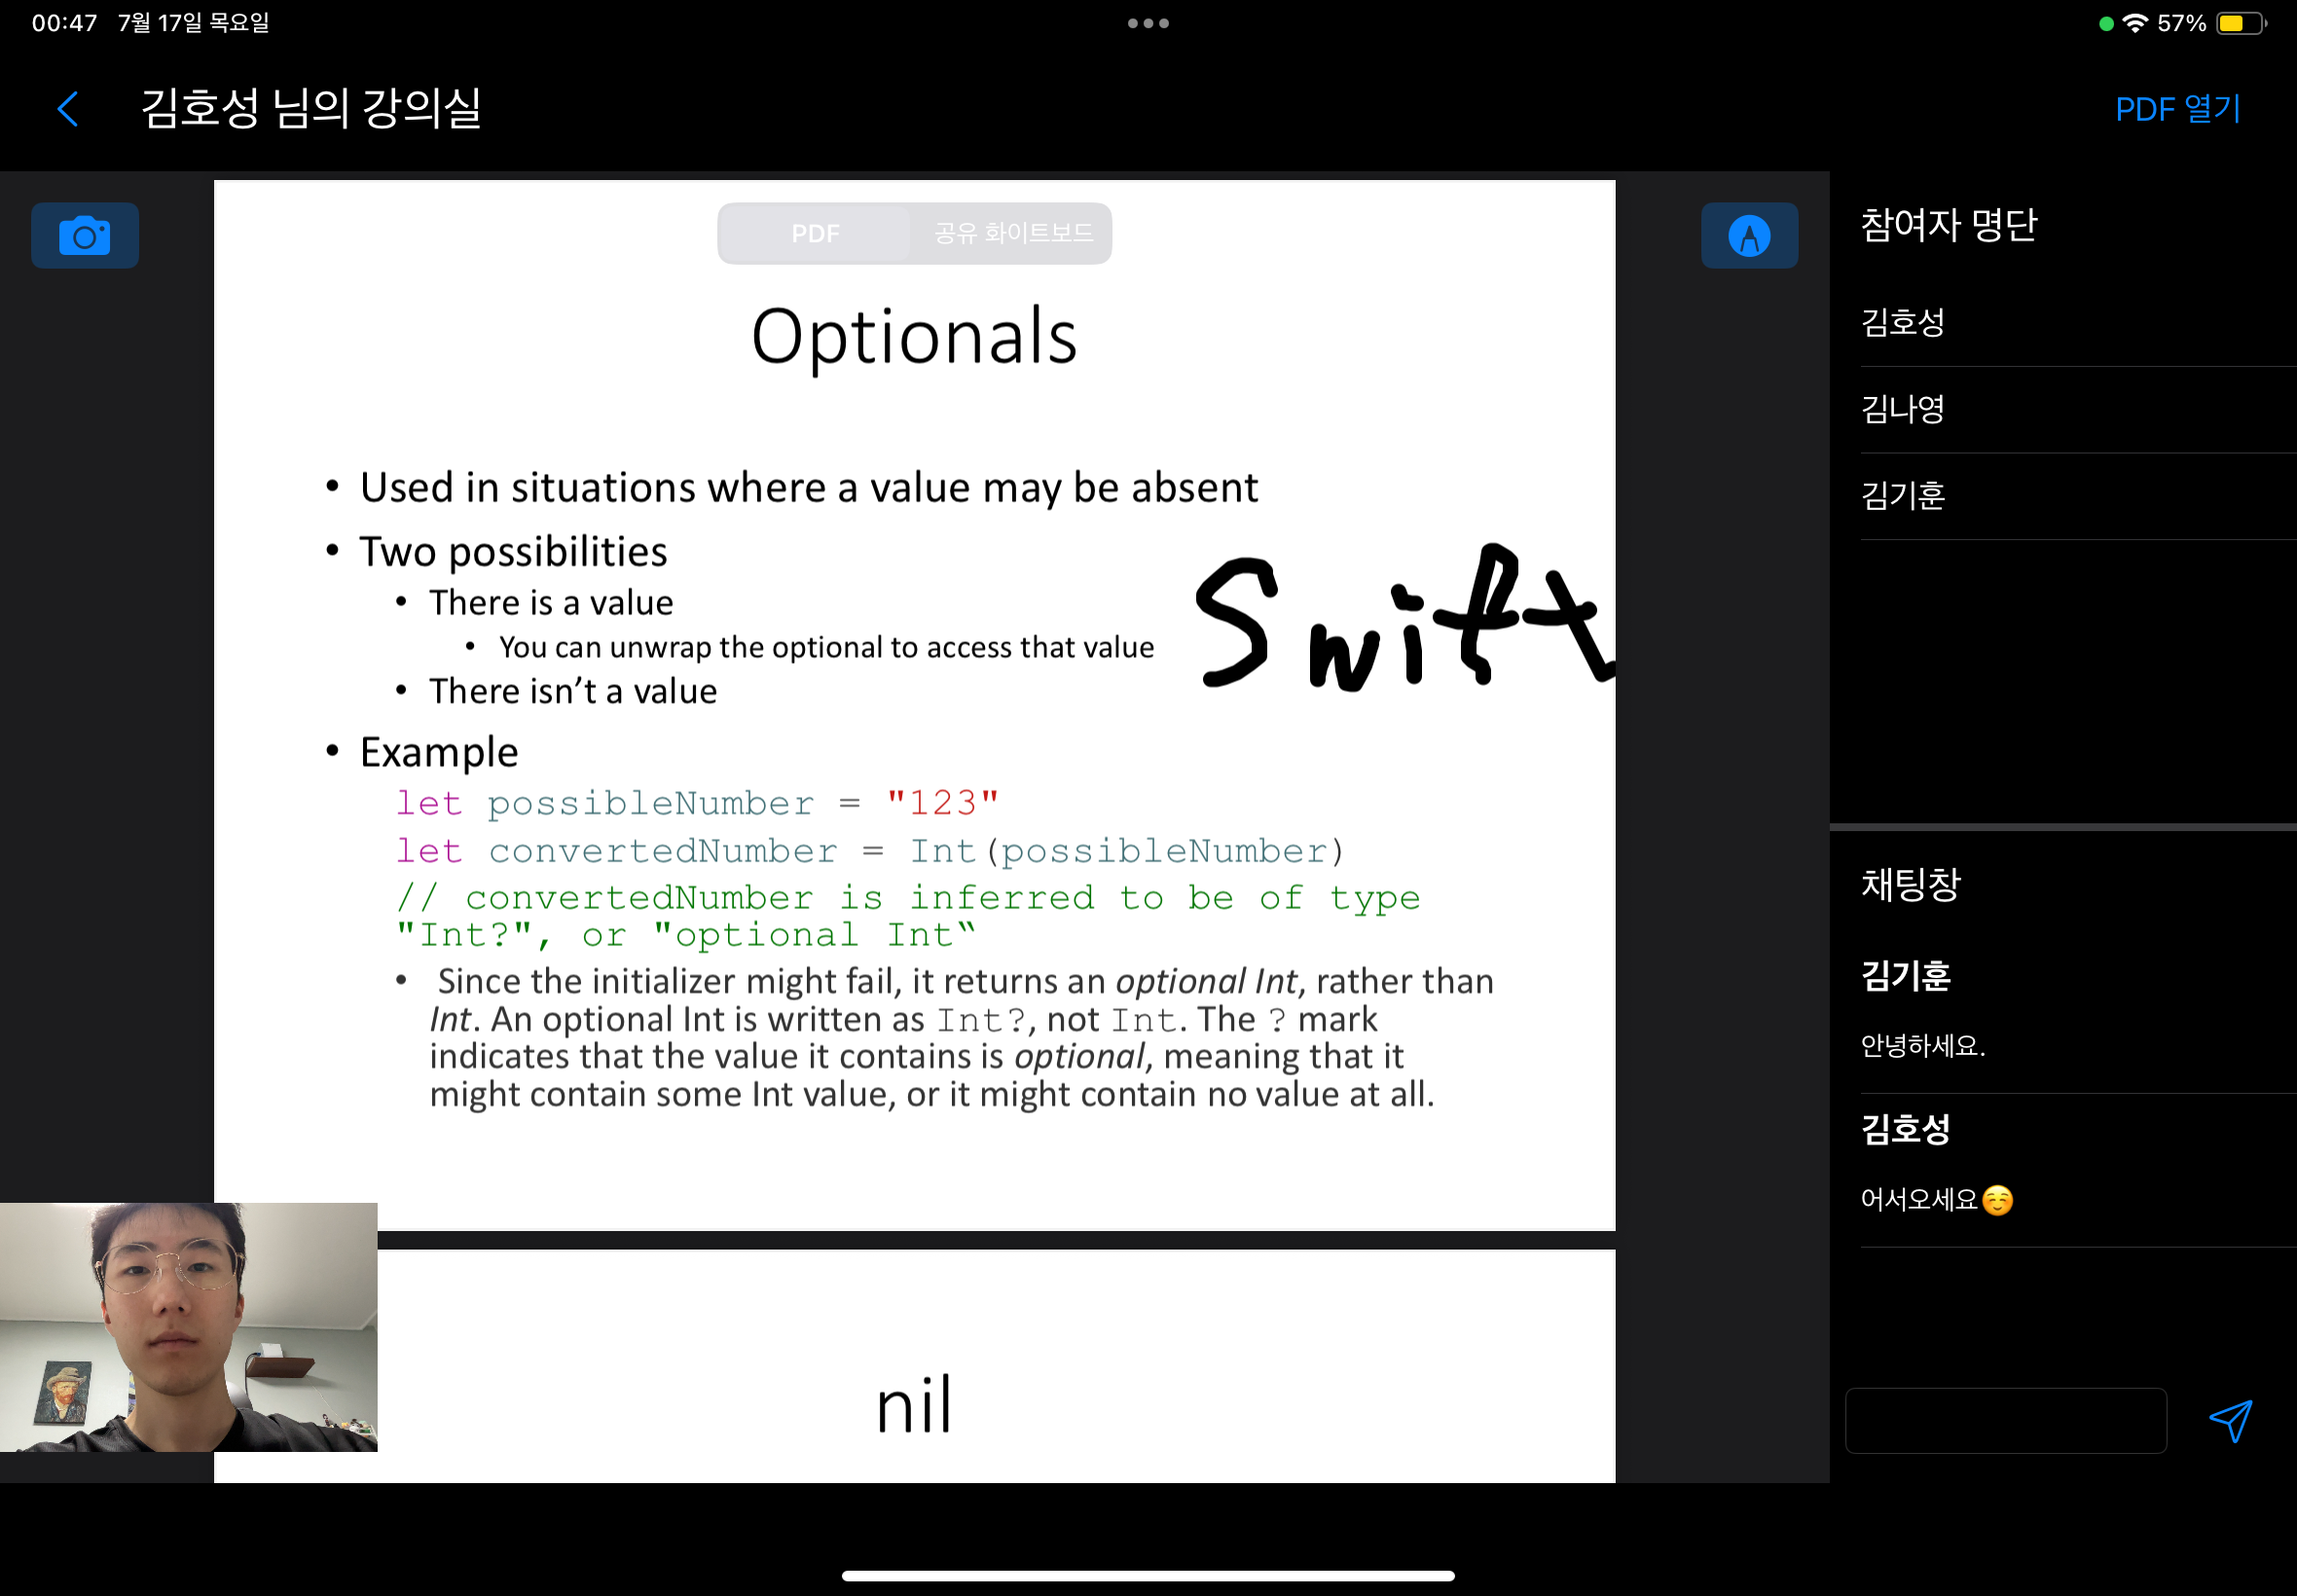
\includegraphics[width=0.9\textwidth]{pdf.PNG}
\caption{User interface of the instructor's client}\label{fig3}
\end{figure}

\begin{figure}[p]
\centering
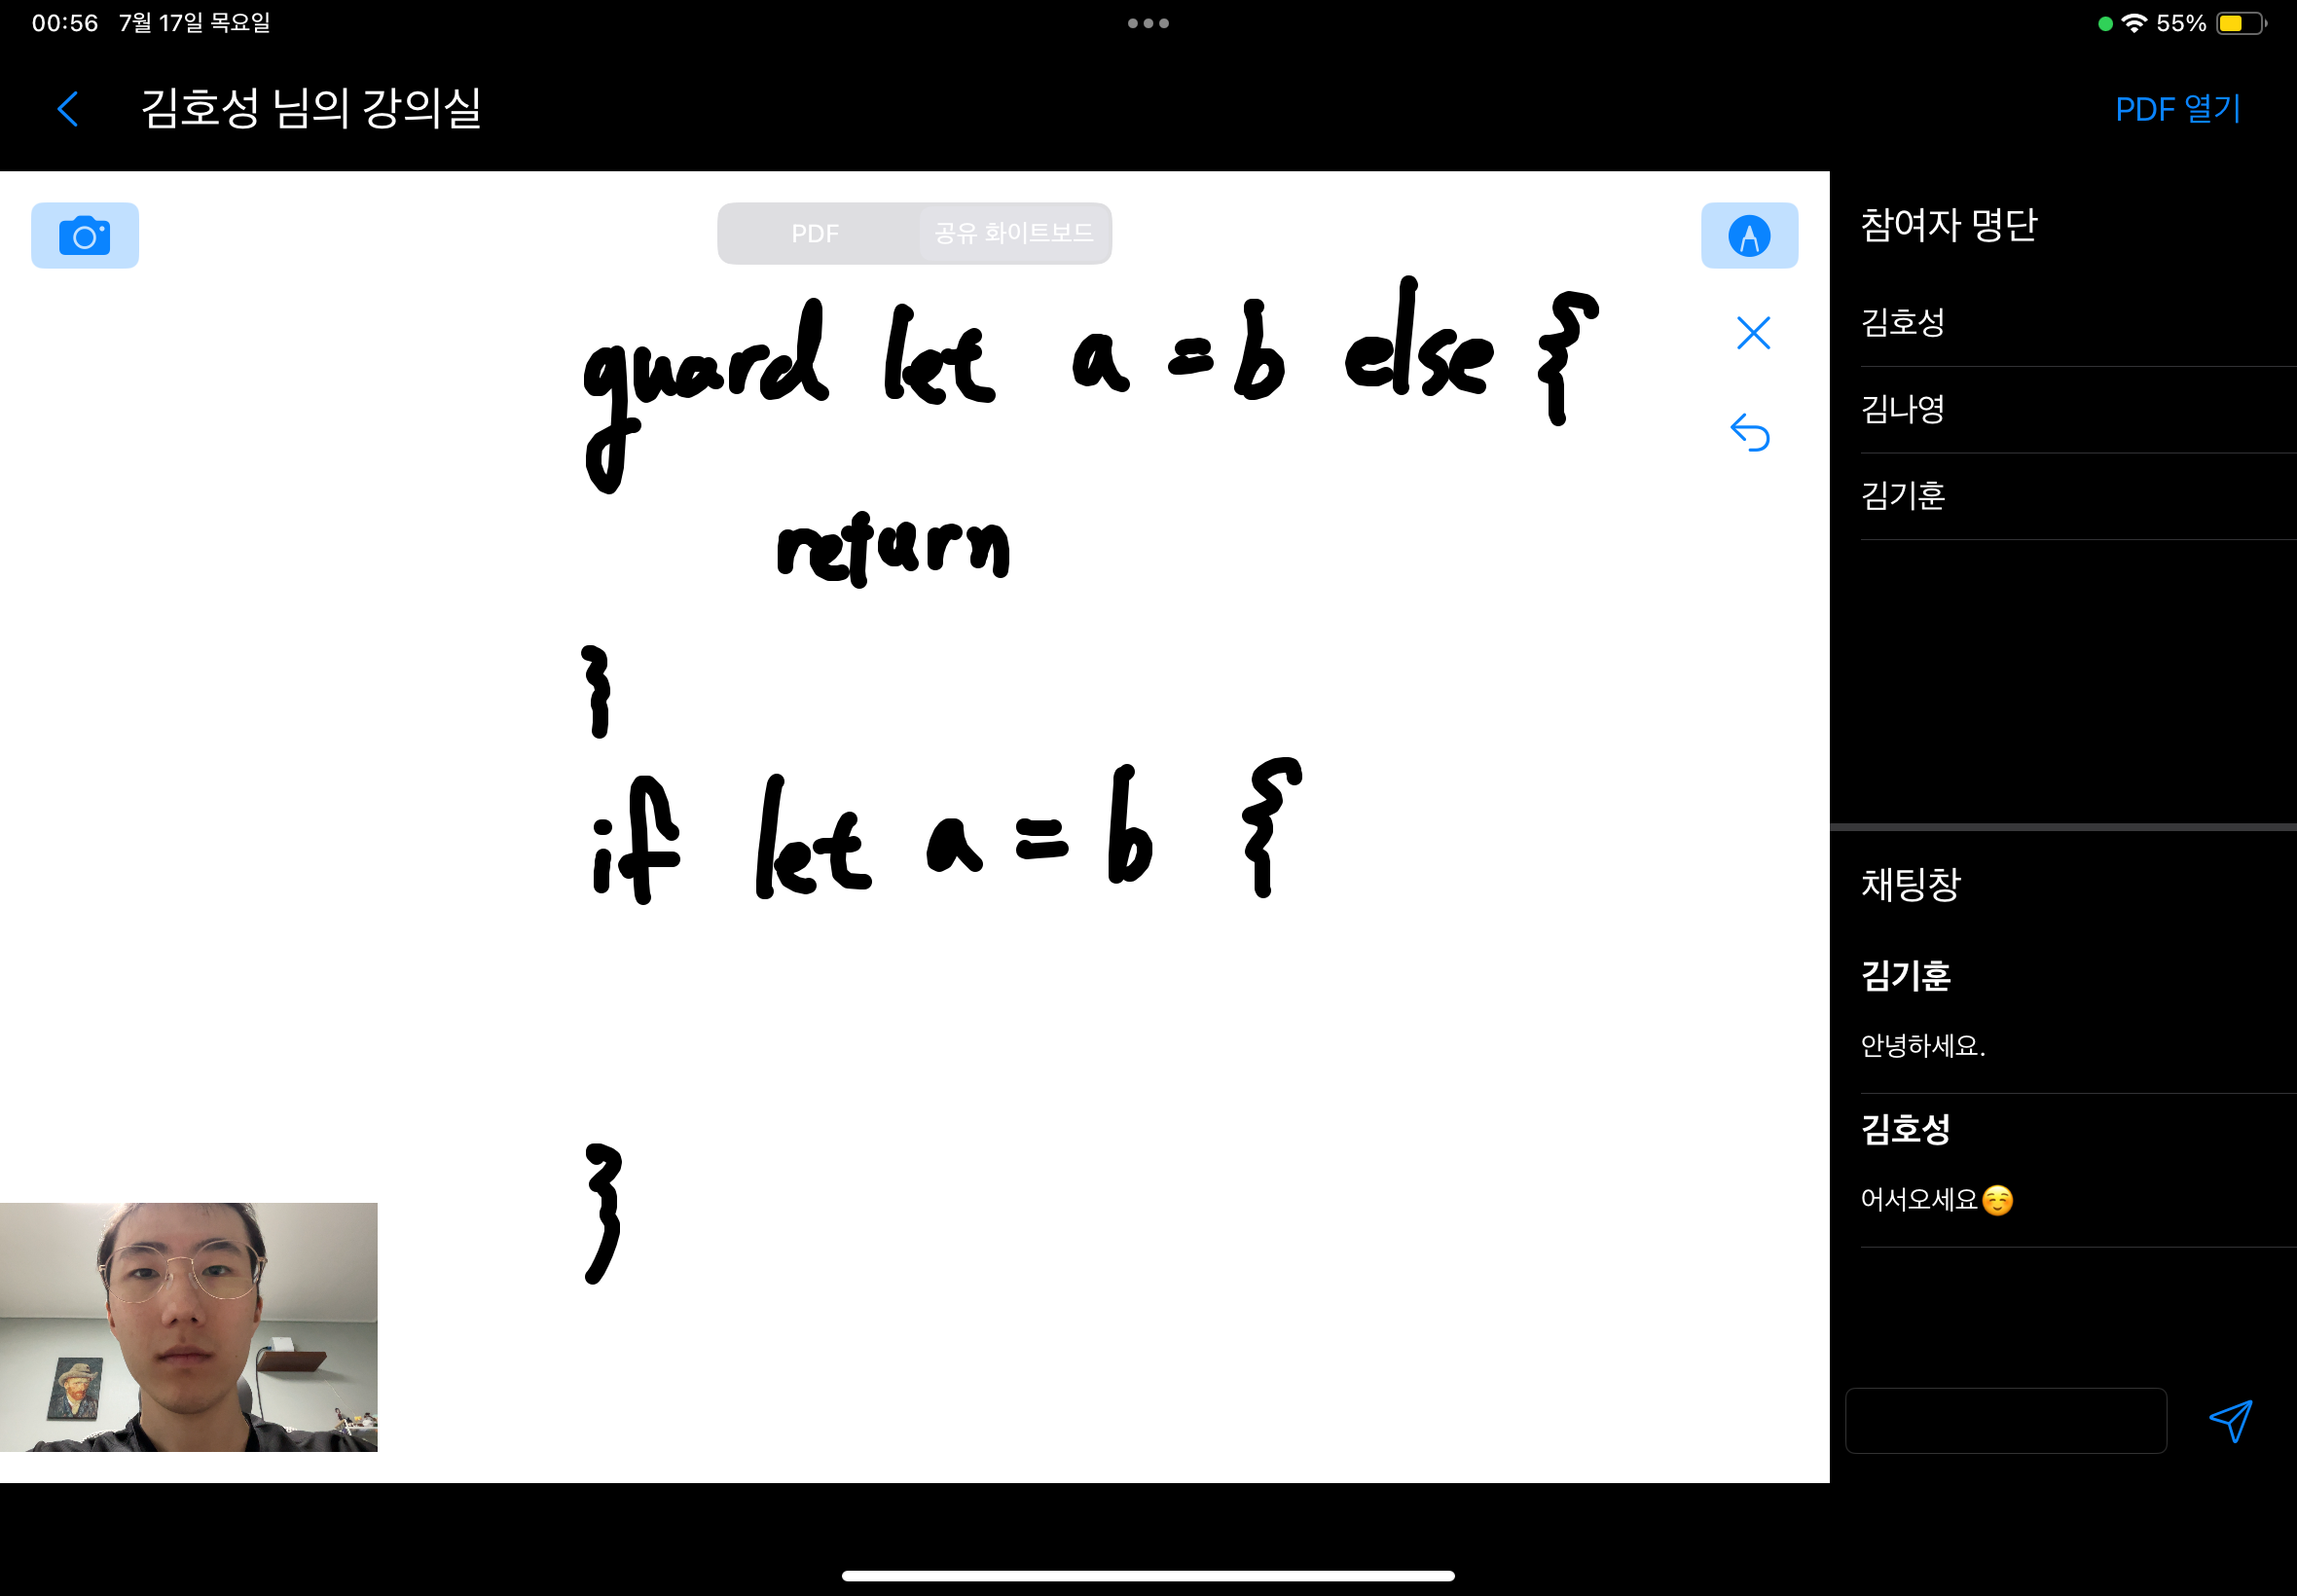
\includegraphics[width=0.9\textwidth]{whiteboard.PNG}
\caption{User interface of the student's client}\label{fig4}
\end{figure}

클라이언트는 기존 단일 강의실 구조에서 다중 강의실 환경으로의 확장, 강의자의 화면 공유 방식의 개선, 접속자 명단 표시, 화이트보드 및 강의자 캠 기능의 추가에 따라 UI 및 내부 로직 전반에 걸쳐 개편이 이루어졌다.

기존 시스템에서는 사용자가 이름을 입력하고 강사 또는 학생의 역할을 선택한 뒤, 하나의 고정된 강의실에 입장하는 구조였다. 반면, 개선된 시스템에서는 홈화면에서 현재 활성화된 강의실 목록을 조회할 수 있으며, 사용자는 강의실을 새로 생성하거나 기존 강의실 중 하나를 선택하여 입장할 수 있도록 변경되었다. 홈 화면의 유저 인터페이스는 그림\ref{fig2}와 같다.

강의자 화면 공유 방식에도 개선이 이루어졌다. 기존에는 전체 화면을 송출하였으나, 개선된 시스템에서는 강의자료가 위치한 특정 영역만을 추출하여 전송한다. ReplayKit\cite{ReplayKit}은 기본적으로 전체화면의 \verb+CMSampleBuffer+만을 제공하므로, 선택 영역 송출을 위해 \verb+CMSampleBuffer+를 \verb+CIImage+로 변환한 뒤, 특정 뷰 영역만 잘라낸 후 \verb+CIContext+에 렌더링하여 \verb+CVPixerBuffer+로 변환하였다. 최종적으로 이를 \verb+CMSampleBuffer+로 변환하여 서버로 송출하였다.

기존 시스템에서는 강의자가 자신의 캠 영상을 확인할 수 없었으나, 전면 카메라의 영상을 \verb+AVCaptureVideoPreviewLayer+를 활용하여 실시간으로 렌더링함으로써 강의자가 자신의 영상 상태를 직접 확인할 수 있도록 하였다.

또한 현재 강의실에 접속 중인 사람들의 명단을 확인할 수 있다. 서버로부터 수신되는 Participant Updated 메세지를 구독하여 참여자 목록을 실시간으로 갱신한다.

화이트보드 기능은 기존 PDF 주석 기능에 사용되었던 \verb+CanvasView+를 활용하여 구현되었다. \verb+CanvasView+는 터치 이벤트를 통해 \verb+UIBezierPath+를 생성하고 이를 배열에 저장하는 방식으로 동작하며 undo, clear 등의 기능도 지원한다.

\section{Conclusion}\label{sec4}

본 보고서에서는 기존의 단일 강의실 기반 동기식 모바일 원격 교육 시스템을 다중 강의실 구조로 확장하고, 실시간 상호작용 기능을 강화한 클라이언트 및 서버 시스템을 설계 및 구현하였다. 시스템 통합의 관점에서는, 기존에 분리되어 운영되던 Java Spring 기반 채팅 서버와 NGINX 스트리밍 서버를 Xcode 프로젝트 내에서 Swift 기반으로 통합하여 실행 및 관리를 일원화하였고, WebSocket 서버는 다중 강의실 기능을 포괄적으로 지원하도록 재구현되었다.

클라이언트 측면에서는 홈 화면을 통해 사용자가 강의실을 선택하거나 생성할 수 있는 구조로 개선하였으며, 강의자는 자신의 전면 카메라를 실시간으로 확인할 수 있고, 강의 자료 영역만을 선택적으로 송출함으로써 화면 공유의 효율성을 향상시켰다. 이외에도 접속자 명단 실시간 확인, 화이트보드 기능을 추가함으로써, 강사와 학생 간의 실시간 상호작용 범위를 실질적으로 확장하였다.

그러나 실제 강의 현장에서는 강의 자료와 칠판이 동시에 제시되는 반면, 본 시스템에서는 PDF 강의자료와 화이트보드를 동시에 시각적으로 제공되지 않는다. 이는 학습자 경험 측면에서 실제 강의 환경에 비해 정보의 병렬적 제공이 제한된다는 점에서 개선이 필요한 부분이다. 향후에는 이러한 한계를 해소하기 위해 두가지 정보를 동시에 표시할 수 있는 UI 구성 방식에 대한 탐색할 예정이다.

전체 소스코드는 \url{https://github.com/H0sungKim/CollaborativeComputingLab}에서 확인할 수 있다.

%===========================================================================================%%
%% If you are submitting to one of the Nature Portfolio journals, using the eJP submission   %%
%% system, please include the references within the manuscript file itself. You may do this  %%
%% by copying the reference list from your .bbl file, paste it into the main manuscript .tex %%
%% file, and delete the associated \verb+\bibliography+ commands.                            %%
%%===========================================================================================%%

\bibliography{bibliography}

\end{document}
